\vspace{0.5cm}
\chapter{Instrumentation, site and infrastructure}

\section{Detector instrumentation}
\label{chap:Detector}

{\begin{wrapfigure}{r}{0.4\textwidth}
\vspace{-0.5cm}
%\begin{figure}{H}
	\centering
		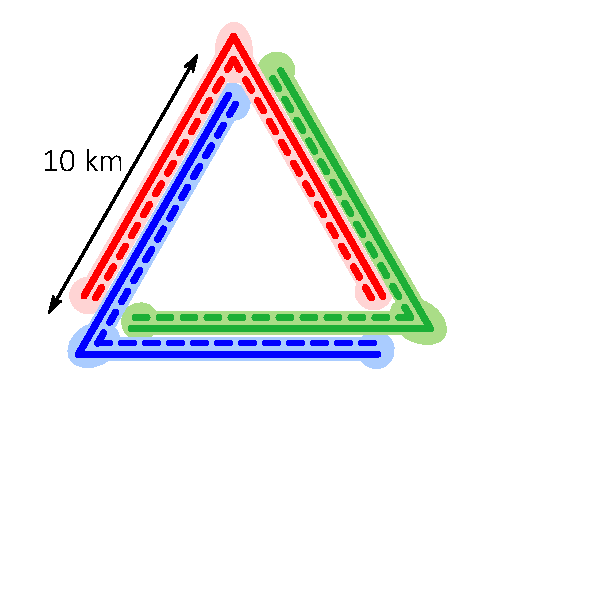
\includegraphics[width=0.35\textwidth]{Figures/ET_simpleB.pdf}
	\caption{The Einstein Telescope will consist of three nested detectors (blue, green, red) in a triangular arrangement. Each detector consists of two interferometers, one optimised for low (solid) and one for high frequency sensitivity (dashed).}
	\label{fig:NestedDetectors}
\end{wrapfigure}

The Einstein Telescope will be a new gravitational wave observatory with a unique design.
A project of this scale must be based on well proven and
experimentally tested technologies. On the other hand, to achieve the sensitivity that the Einstein Telescope
project aims for, it will be necessary to exploit many
state-of-the-art technologies and drive them to their physical limits.
The Einstein Telescope combines the proven concepts from current 
detectors such as LIGO and Virgo with advanced upgrades,
such as cryogenic mirrors, in a infrastructure designed to 
accommodate several technology upgrades over a period of 50 years.

\subsection {Optical Layout and Interferometery}
% Authors A. Freise
\label{Sec:Layout}

The Einstein Telescope aims at providing a significant increase in scientific 
reach through a tenfold improvement of the detector sensitivity in a wide
frequency band, and, in addition, by extending the range of the detector
to lower frequencies. 
The overall improvement can only be achieved by significantly increasing the
length of the detector beyond the size of currently available instruments (i.e.\
3\,km for advanced Virgo and KAGRA, and 4\,km for advanced LIGO) and going to an
underground location, where the seismic noise, and hence the level of gravity
gradient noise, is lower than at the surface. 


By increasing the arm length to 10\,km the influence of unavoidable displacement
noises can be lowered to allow a significant improvement in sensitivity, in
particular at low frequencies. Observing gravitational waves at frequencies well
below the limits of current detectors will also require advanced technologies
such as cryogenic mirrors and active noise cancellation.

The Einstein Telescope is a single-site observatory that will consist of three
nested detectors, arranged in a triangular pattern as shown in 
figure\,~\ref{fig:NestedDetectors}. 
}

The triangle shape, similar to the space-based LISA detector, represents the smallest layout for a single-site observatory that is equally sensitive
to both polarizations of the gravitational wave signal. It also provides
redundancy for continuous data taking during maintenance or upgrades of a single detector, and has the potential for exploiting elaborate data analysis techniques developed for LISA such as null-streams for noise identification and removal.

\subsubsection{A Configuration Covering Multiple-Spectral Bands}

In contrast to all currently existing detectors, each of the three ET detectors will be composed of two interferometers, one specialized for the detection of low-frequency gravitational waves and the other for high-frequency waves. The sensitivity goal for each interferometer is shown 
in figure\,\ref{fig:ET_sensitivity}. This so-called \textit{xylophone}
configuration separates the high laser power required for good high-frequency performance from the cryogenic mirror suspension systems employed for a good low frequency sensitivity into two separate, parallel systems.
In order to achieve a sufficient sensitivity at high frequencies the light power in the arms of the high-frequency interferometer needs to be in the megawatt range. Thermal noise considerations on the other hand require cryogenic optics to reach the sensitivity goal at low frequencies. 
Operating cryogenic optics at a level of several megawatts of light power presents a serious technological challenge that is extremely hard to master. 
Even for the best mirrors that state-of-the-art coating technology can produce, the residual absorption of only about one ppm leads to an absorbed power of several watts at a circulating light power level in the megawatt range. 
The resulting thickness of the suspension fibres, which would be needed to remove the heat, would spoil the performance of the ultra low loss suspension. 
The interferometer dedicated to detecting high-frequency gravitational waves (ET-HF) in the range from about 30\,Hz to 10\,kHz will be operated at room temperature, will use fused silica optics with a diameter of about 60\,cm and a mass of about 200 kg each, will have a light power of about 3\,megawatts in the interferometer arms, and will run with an interferometer configuration optimized for high frequencies (tuned Resonant Sideband Extraction). 
The cryogenic, low-frequency interferometer (ET-LF), operated at a temperature of 10\,K and aimed at the frequency range from 1.5\,Hz to 30\,Hz, will use signal recycling tuned to maximise low-frequency sensitivity, will have a light power of 18\,kW  in the interferometer arms, and silicon mirrors with a diameter of about 45\,cm and a mass of about 200\,kg. 
%\begin{wrapfigure}{r}{0.6\textwidth}
\begin{figure}[ht]
	\centering
		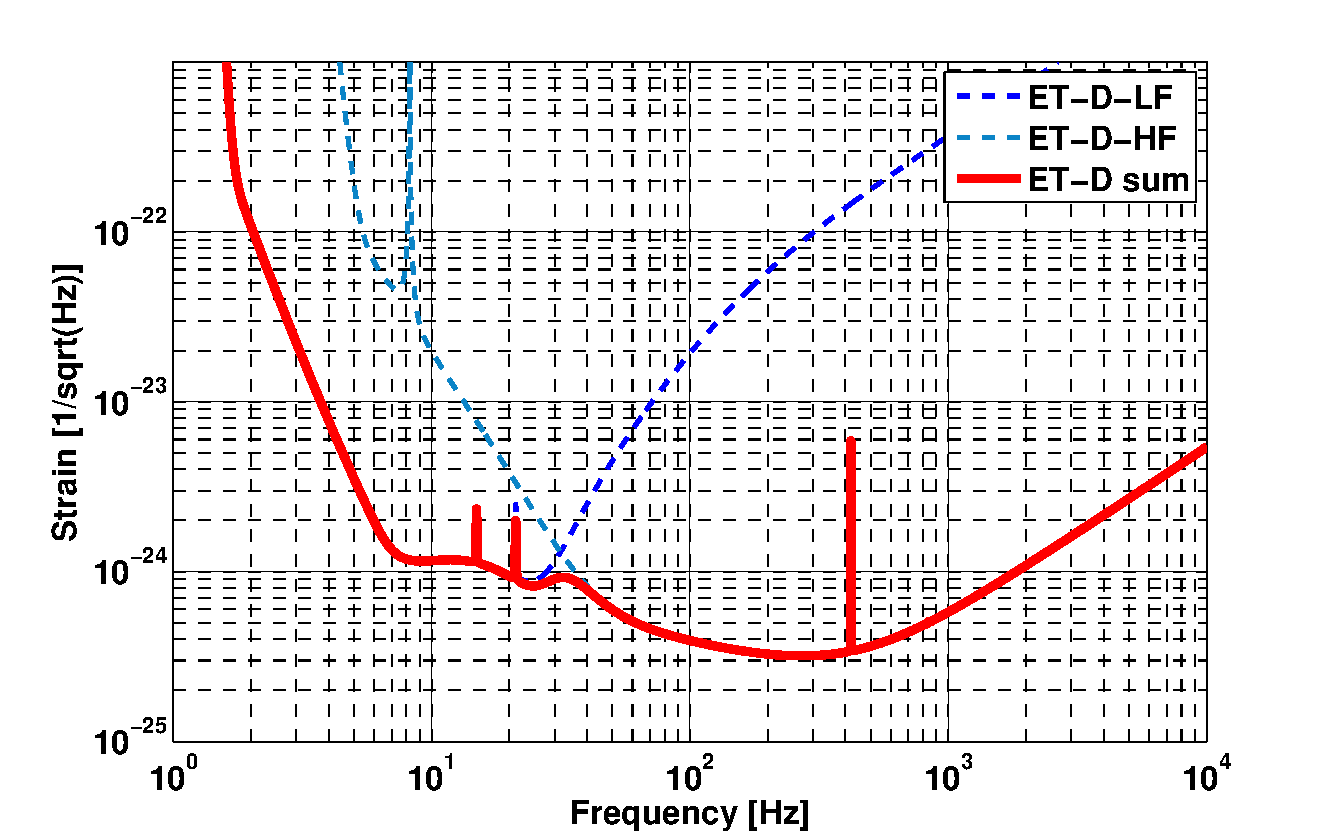
\includegraphics[width=0.6\textwidth]{Figures/ET_D_spectrum.pdf}
	\caption{Sensitivity of the Einstein Telescope. 
	%in the `xylophone' configuration. 
	% comment sth: deleted the last few words as it seemed to suggest that there also are other configurations than the xylophone.
	The sensitivity of the low-frequency cryogenic interferometer is shown in the 
	dashed dark blue curve and the one of the high-frequency room temperature 
	one in a dashed blue-green tone. The resulting total detector sensitivity is
	shown as the solid bright red curve.}
	\label{fig:ET_sensitivity}
%\end{wrapfigure}
\end{figure}

The xylophone configuration addresses two other challenges as well:

\textbf{Control Noises}: Many noise sources limiting the second generation GW detectors at the low frequency end become more challenging with increased optical power: classical radiation pressure forces and torques originating from residual misalignments and beam jitter dominate the dynamics of the interferometer mirrors and hence the local and global control loops. 
The xylophone concept will help ET to achieve its unprecedented low-frequency sensitivity target, by minimising the radiation pressure driven forces on the mirrors of the ET-LF detector.

\textbf{Shot Noise vs Radiation Pressure Noise:} Due to the fact that the shot noise contribution scales inversely with the square root of the optical power, but the photon radiation pressure noise contribution on the other hand scales proportional to the square root of the optical power, it will be hard to obtain the desired bandwidth with a single detector.
The xylophone allows us to optimise quantum noise through operating the high and low frequency interferometers at very different optical powers.

\subsubsection{Core Optics}
%  Author: Jerome
\label{Sec:CoreOptics}
The core optics are the four main mirrors making up the Fabry-Perot arm cavities and are the heart of the ET interferometers.
To ensure the best optics, the three ingredients of a mirror, i.e. substrate,
polishing and coating, must be manufactured using state-of-the-art technology. The temperature at which the mirror is operated has a strong impact on the technological choices to be made.
ET will require larger mirrors than current generation detectors. The large mirror mass will not only reduce radiation pressure effects but will also allow us to use larger sized beam spots on the mirror surfaces for lowering thermal noise  effects. 

\textbf{The mirror substrates} must meet some demanding specifications in terms of optical and mechanical specifications, and should be available in large sizes with surfaces polished to sub-atomic level accuracy. Due to these constraints, only a few specific materials are considered: special grades of fused silica for room temperature interferometer and ultra-pure silicon for cryogenic temperatures.
% comment sth: I added some adjectives to indicate that the reader understands already here that it is not any fused silica or any silicon we can use, but within these materials we still have very specific requirements like Suprasil 3001 or floatzone/magnetic CZ silicon.

Fused silica
is the substrate of choice for all the current room temperature interferometers.
Due to its use for first and second generation gravitational wave detectors, this material has been extensively characterised at room temperature.
Moreover the polishing and coating technologies are now highly developed for this material.
Serving as a pathfinder for ET, the upgrade of Advanced Virgo, called Advanced Virgo+ will use fused silica test masses with a diameter of  55\,cm and a weight of 100\,kg. 

Silicon is the preferred candidate material for the test masses for the cryogenic ET low-frequency interferometers. 
Unlike fused silica, silicon is not transparent at a laser wavelength of 1064\,nm and so the operating wavelength of the LF interferometers has to be shifted to 1550\,nm. 
In contrast to fused silica, silicon has excellent mechanical and thermal properties at cryogenic temperatures and is easily available in relatively high quality due to the large market of the semiconductor industry.
%The coefficient of thermal expansion is zero at two special
%temperatures around 18~K and 125~K \cite{lyon1977siliconexpansion}. At these
%temperatures the contribution of thermo-elastic noise will therefore vanish. 
%
%It was
%experimentally shown that silicon bulk samples can reach mechanical losses as
%low as $1 \times 10^{-9}$ at 10~K. \cite{mcguigan1978siliconQ}.
The maximum available diameter and purity of silicon depends on the fabrication
process. The two main growing processes for single crystal silicon used by the
semiconductor industry are the Czochralski (CZ) and the Float Zone (FZ) methods.
CZ silicon is grown from a silicon melt in a fused silica crucible, resulting in relatively large samples with reasonable purity. 
%The most dominant impurities
%in undoped CZ-grown silicon are carbon (typically 10$^{-18}$ cm$^{-3}$) and
%oxygen (typically up to 10$^{-19}$ cm$^{-3}$). 
In comparison, FZ silicon also contains impurities but in much smaller concentrations (up to 10$^{-3}$ times smaller). 
Using the CZ growth technique, silicon ingots up to 45~cm of diameter can be produced though 30\,cm is still the dominant wafer diameter in the semiconductor industry. For FZ silicon the diameter is currently limited to 20\,cm.
In the recent years the optical properties of silicon have been thouroughly characterised. According to the latest measurements, the magnetic Czochralski (mCz) growth technique is the most suitable approach for ET as it can combine large diameter ingots (45\,cm diameter) with very low impurities and absorption at the 20\,ppm/cm level. These level of absorption are promising but further developments are required, and the effects of residual birefringence intrinsic to crystalline materials have to be evaluated.
%has been achieved on one sample.
A backup substrate choice could be sapphire as a candidate material for ET-LF. Sapphire is already used in the Japanese cryogenic interferometer KAGRA, though much smaller in size than what is required for ET, and hence extensive experience has been acquired on operating those mirrors  in cold conditions.% \cite{Akutsu_2019}. 
Like for silicon, large sapphire boules with excellent optical properties still have to be demonstrated.

\textbf{Polishing of the surfaces} of fused silica substrates is well mastered
thanks to the current generation of room temperature interferometers as well as EUV
lithography optics and hence presents minimal risks. For the Einstein Telescope
main mirrors, the already-demonstrated surface quality such as surface
height errors below 0.3\,nm RMS for low spatial frequencies (flatness) and below\,0.1 nm
RMS for the roughness (smaller defects) will be enough, albeit it must be
achieved on a larger area since the ET mirrors will be bigger.

Polishing of silicon does not carry any difficulties as this substrate material is heavily used for X-ray mirrors, but demonstrator meeting all the ET polishing specifications will have to be produced. Experiences from polishing companies indicate that silicon could be polished the same way as fused silica and similar surface figure accuracy and roughness can be achieved (using also ion beam figuring to reach sub-nanometer flatness). The very low roughness is more challenging but 0.2\,nm RMS could be achieved and is acceptable for ET. 
%Andreas: The number comes from Jerome
%\todo[inline]{Not sure where this number comes from and about the fact that excellent micro-roughness is harder to achieve. I do not think that we would be happy with 0.2nm micro roughness even now for advanced optics... "roughness" per se is ill defined without saying which spatial frequencies we are talking about. Currently achievable values for surface figure errors are limited by the measurement capabilities and range in the 50 pm rms range.}

\textbf{Thin optical coatings}, a few microns in thickness, must be added to the surfaces of the mirrors to make them highly reflective for the used laser wavelength. 
Since the thermal noise from these coatings will limit the sensitivity of current room-temperature detectors at their most sensitive frequencies, it is essential to reduce coating thermal noise to achieve the ET design sensitivity.
To meet the goal of a factor of 25 improvement in sensitivity over Advanced LIGO design sensitivity at 10 Hz, ET-LF requires a reduction in coating displacement thermal noise by at least a factor of 10 with respect to Advanced LIGO.
Some of this improvement can be obtained from operating at low temperature and through the use of larger laser beam spots on the mirrors.
The target for ET-HF is a factor of 3.2 reduction in coating thermal noise
amplitude spectral density (ASD)
at 100 Hz compared to Advanced LIGO design sensitivity. Accounting for the slightly
larger laser beam in ET-HF, this sets a requirement of a reduction in ASD by a
factor of 2.7 from the coating materials. If we assume all coating properties
except the mechanical loss remain identical, then a reduction in mechanical loss
by a factor of 7.1 with respect to the Advanced LIGO coatings would be required.

Significant progress has been made towards development of coatings suitable for low temperatures in ET-LF. There are several highly-promising routes to meeting the coating thermal noise and optical absorption requirements. 
However, further studies are required optimising the trade-off between coating absorption requirements, suspension thermal noise, ultimate mirror temperature and substrate thermoelastic noise.
% – and it seems likely that lower absorption than 5 ppm may be required.
Achieving significant reductions in coating thermal noise at room temperature
may be more challenging than at low temperature. Work in this area is ongoing,
both for ET and for upgrades to the Advanced LIGO and Advanced Virgo detectors.
%, and there are several promising avenues which are currently being investigated. 

\subsubsection{Michelson interferometer}

Each individual interferometer has a classical dual-recycled Michelson topology with arm cavities. This is a mature technique, well tested by  
second-generation detectors, Advanced LIGO and Advanced Virgo. More elaborate topologies like Sagnac interferometers fit equally well into the planned infrastructure but are not considered for the initial installation, as they have not yet reached the required level of maturity.

Each of the ET interferometers will require a novel high power laser system with
low intrinsic noise called the high power laser (HPL) in the following. 
The ET-HF HPL has to operate in a single-frequency continuous-wave (cw) mode at a wavelength of 1064\,nm and needs to deliver 700\,W in a linear polarized fundamental spatial HG$_{00}$ mode. With the assumption of roughly 30\% loss in the injection path this leaves 500\,W at the input of the main interferometer. The higher order mode content of this laser should be below 10\% and the polarization purity at least 1/10. 
The ET-LF HPL needs to operate in a single-frequency continuous-wave (cw) mode at a wavelength of approximately 1550\,nm with similar spatial and polarization purities as the ET-HP HPL. This different wavelength for ET-LF follows from the material choice for the test masses.
A laser power of 5\,W is required to allow for 3\,W to be injected into the main interferometer. Both laser systems have to achieve demanding noise requirements for all frequencies in the observation band:
a frequency noise in the $10\,\mathrm{mHz} / \sqrt{\mathrm{Hz}}$, relative lateral
and angular beam fluctuations in the $10^{-6} / \sqrt{\mathrm{Hz}}$ range
and a laser power stability of roughly RPN $= 3\!\times\!10^{-10} /
\sqrt{\mathrm{Hz}}$. These requirements appear to be feasible using current approaches to stabilization.

Advanced detectors have recently been upgraded with \textit{squeezed light} which generates correlations between the phase and the amplitude quadratures. In the shot noise  dominated frequency range squeezed light is used which shows lower phase fluctuations (at the cost of the amplitude fluctuations) in comparison to classical  laser light in the interferometer arms. In the low-frequency, radiation pressure dominated range the fluctuations need to be lowered in the amplitude quadrature. 
%This goal can be 
Providing the right spectral dependence of the so-called \textit{squeezing angle} can be  achieved by reflecting squeezed light off a filter cavity. 
For the ET we assume 15\,dB initial squeezing level at the squeezing source and an effective squeezing level of 10\,dB to be 
available (equivalent in shot noise reduction to a laser power increase of a factor
of 10). 

The squeezing level, and with it the sensitivity improvement that can be reached, 
depends on the optical losses in the squeezer, the filtering optics, the interferometer, 
and all optical devices on the way to the photodetector, including the photodetector 
efficiency itself. It will therefore be essential 
to keep the optical losses as low as possible. 
These levels of squeezing, and maintaining the low losses required to preserve the squeezing, will require technology development.
%Optical losses of 75\,ppm per round 
%trip are currently achievable with state-of-the-art techniques and are used as a 
%conservative estimate for the filter cavities.


\subsection{Seismic Isolation and Suspension}
% Authors: Giovanni Losurdo, Giles Hammond, Conor Mow-Lowry
\label{Sec:SASandSUS}
%\subsection{Seismic Isolation System}


Seismic isolation refers to the stage(s) of isolation systems closest to the ground. It fulfills two main
functions: to suppress the seismic noise below the sensitivity requirements in the detection frequency range
(for ET at frequencies larger than 1-2\,Hz); and to reduce the RMS input motion to the suspension systems,
particularly at the suspension resonances and the micro-seismic peak(s). It also provides large-scale and
slow position control of the test-masses.

The baseline for ET, originally defined in the 2011 ET conceptual design report, consists in using a longer Virgo-style
Superattenuator. The increased length (17\,m) reduces the normal mode frequencies, pushing
the seismic wall down to $\sim 2$\,Hz. The main advantage for such a choice is that it employs a design
thoroughly tested during many years of operation in Virgo and it requires relatively little R\&D to be
adapted to ET. It therefore represents a safe pathway towards a 3G configuration.

A possible alternative to be investigated via a dedicated R\&D program is the
coupling of a Superattenuator to an inertial platform controlled in all 6
degrees of freedom. 
This configuration would make use of a combination
of technologies and expertise developed in the GW field in the last decade. The
inertial platform would support the Superattenuator, an approach that was
envisaged for use in Virgo. The Superattenuators are supported on a rigid
platform resting on 3 elastic feet that can be actuated by piezo actuators in
order to actively control of the ground tilt. The ET design would extend this concept to also improve horizontal performance.
An advantage of this alternate could be relaxed requirements on the physical infrastructure, providing an advantageous cost and risk trade.

%Such an approach could in principle allow to shorten the Superattenuator height and, consequently, the height of the caverns.
%Comment by stefan: While I completely agree with this statement, I am not sure if this sentence helps our ESFRI application and hence I would advocate to remove the previous sentence for now.)


%\subsection{Test Mass Suspension Systems}
\subsubsection{Thermal noise of the mirror suspensions}
The main requirements of a gravitational wave mirror suspension are to reduce seismic noise input from the ground and to provide a mechanism to steer the mirror via electromagnetic/electrostatic forces for alignment and control. This must all be done while minimising the thermal noise arising from the suspension. Suspension thermal noise arises due to mechanical dissipation in the materials which make up the suspension (Brownian noise) or through thermoelastic noise, the coupling of statistical temperature fluctuations through the thermo-mechanical properties of the suspension materials such as the thermal expansion coefficient and the Young's modulus. \\
{\bfseries High Frequency Suspension}: The current room temperature
interferometers (Advanced LIGO, Advanced Virgo, GEO) utilise fused silica as a material to
suspend the test masses. The suspensions were initially pioneered in GEO
around 1990-2000 (5.6~kg optics),  upscaled for use in Advanced LIGO and Advanced Virgo (both
40~kg optics) between 2000-2012, with installation occurring from 2015 onwards.
Fused silica is the material of choice as it can be pulled into long thin
fibres, can be welded to form monolithic structures, has extremely low internal
friction,  and has a breaking strength in excess of 4~GPa. The ET-HF
suspension mirror mass will be increased to 150~kg - 200~kg to provide lower
suspension thermal noise and also reduction of radiation pressure noise. There
is a mature technology in place to deliver the technology for a room temperature suspension, building on many years of heritage and proven technology in the field. The Heraeus Suprasil family of synthetic glasses will be utilised, and initial work has shown that fibres of suitable geometry can be pulled and
welded. While the fused silica solution is already well developed, there needs to
be work devoted towards the demonstration of a full scale ET HF prototype. Key
areas of future R\&D include
the testing of a full scale prototype suspension with fused silica fibres with
operating stresses of around 1 - 1.5~GPa;
activities to prove the stress-corrosion properties of fused silica, and the
techniques required to bond/attach the ear/fibres to the test mass; the
demonstration of sensors and actuators with sufficient sensitivity 
%and control authority 
for suspension local control and damping; and the demonstration of mitigating
excess charges in electrostatic actuation.\\
{\bfseries Low Frequency Suspension}: In addition to providing a low seismic/thermal noise platform, the ET Low Frequency suspension also has to fulfill a second crucial duty - to extract the thermal load that is put into the optical component by the laser beam ($\simeq 10 $mW). The materials of choice are crystalline materials that have a very high thermal conductivity at low temperatures and also display low mechanical loss. In particular, both silicon and sapphire are excellent materials in the temperature region of interest (typically below 20\,K). Sapphire has a higher thermal conductivity than silicon below 20\,K. Sapphire fibres for heat extraction have been investigated in detail by Japanese groups for KAGRA. At low temperatures the mechanical loss of the suspension, which defines the thermal noise performance, is a key driver for the suspension design. Heavy test masses will be utilised, with the addition of low temperature to provide enhanced thermal noise performance. Thermoelastic noise drops away sharply with decreasing temperature, and indeed for silicon is zero around 120~K and as $T<20$~K. While sapphire is the baseline for KAGRA, the need for large and heavy test masses (150~kg - 200~kg) highlights silicon as a preferred material for ET-LF.  Silicon suspension elements are currently under investigation in the form of fibres and ribbon-like geometries. Fabrication techniques include (i) Laser Heated Pedestal Growth, (ii) micro pull down and (iii) etching from wafers. R\&D activities are needed on several aspects of the low frequency suspension:
\begin{itemize}
\item fibre fabrication techniques, to develop long thin silicon or sapphire fibres, and to join the suspension elements to the ears and test masses;
\item detailed FEA modeling of the final stage suspension, in order to estimate the effects of real fibre geometries on the thermal noise performance;
\item inertial sensors and actuators, operating at cryogenic temperature, with high sensitivity and large bandwidth; 
\item prototyping the lower stage suspension, including a fast turnaround tabletop systems and small scale prototypes of 10\,m arm length with payload in the 1\,kg to 10\,kg range.%Gianluca: this last point is not clear. It means that we need to build a 10m arm ifo?
\end{itemize}

\subsection{Vacuum System}
% author G.Gemme
\label{Sec:Vacuum}
In laser interferometers for GW detection the instrument has to be kept under High-Vacuum or Ultra-High-Vacuum (HV, UHV) for several reasons: 
\begin{itemize}
\item reduce the noise due to residual gas fluctuations along the beam path to an acceptable level; \item isolate test masses and other optical elements from acoustic noise; 
\item reduce test mass motion excitation due to residual gas fluctuations;
\item reduce friction losses in the mirror suspensions  contribute to thermal isolation of test masses and of their support structures; 
\item contribute to preserve the cleanliness of optical elements. 
\end{itemize}
The power spectral density of gas-induced fluctuations in the optical path length has been calculated choosing conservative beam shape parameters and taking a safety factor of at least $10$ with respect to the pressure producing a phase noise at the limit of the best sensitivity for the ultimate detector envisioned for ET.
The residual gas composition will be dominated by hydrogen with presence of water and other gases; we will keep the total residual pressure at about $10^{-10}$~mbar, corresponding to a noise level below $10^{-25}$~Hz$^{-1/2}$.
The vacuum system will be extremely clean from heavy organic molecules, both to limit the phase noise and to prevent pollution of the optical components. Hydrocarbon partial pressure shall be at the level of $10^{-14}$~mbar.

The technologies that were developed and employed in the existing gravitational wave observatories have been shown to meet the stringent requirements of vacuum integrity, very low hydrogen and heavy molecule outgassing, minimal particulate generation, low vibration, and appropriate stray light optical absorbance for successful operation. However, straightforward extrapolation of the costs for extending the interferometer vacuum beam enclosures from the current lengths of 3-4~km/arm to $\sim10$~km/arm indicates the need for investigation of a range of technologies and materials that could significantly lower the final cost, facilitate construction and increase the life-cycle operation of vacuum systems for next generation observatories. 

\begin{comment}

The baseline choice for the material of the vacuum enclosure is stainless steel (304L), based on the experience of first-generation installations. Two alternative options are a low carbon, mild steel alloy and aluminum that could both offer significant cost savings. Regarding these options, some open issues need to be studied and clarified. These include choice of the mild steel alloy, potential surface treatments or coatings for the mild and stainless steel and the aluminum alloy, and the cost of incorporating the many transition elements (flanging and expansion joints) if aluminum is chosen as the base vessel material.

In order to minimize the cost of in-situ bake out systems for removal of adsorbed water following the initial or subsequent exposure to air, a number of potential surface coatings are being investigated for stainless and mild steels including TiC, diamond-like carbon (DLC), amorphous Silicon (a-Si) and a class of conversion coatings such as magnetite (Fe$_3$O$_4$) that could be applied during the mill processing of the steel (so-called conversion coatings). A number of characteristics of these coatings were identified for further study before their cost effectiveness could be quantified including additional H$_2$O adsorption studies, coating deposition costs at scale, film toughness, particulate generation, interference with vessel welding, and optical characteristics.

Viable first order pumping schemes are being considered. Specific pump-down routines were identified from atmospheric pressure to UHV using pumps that would minimize or eliminate hydrocarbon or particulate contamination. The continued use of large area liquid nitrogen panels is recommended based on the high-water pumping speed and satisfactory performance in current generation systems. UHV performance can be maintained with periodically spaced getter pumps and ion pumps. The availability of the new getter alloy from SAES (ZAO) is particular useful for this application because of its large pumping speed and capacity for H$_2$O and H$_2$. In addition, conventional titanium sublimation pumps (TSP) are not ruled out for consideration.

The use of clean, ultra-dry (ppb water), warm gas purging systems could significantly affect the need for in-situ bake-out systems for removal of adsorbed water following the initial or subsequent pump-downs from atmospheric pressure. The incorporation for such systems for the first-generation gravitational wave observatories can significantly shorten downtime in the event of a loss-of-vacuum incident.

Finally, the value of partnerships with industrial contractors with relevant expertise was demonstrated by the successful design, installation and operation of current installations. Such partnerships can be valuable in the pre-competitive phase to test the viability of the proposed concepts and they are certainly valuable in the final design and early constructions phases to test prototypes of full vessel segments.

\end{comment}

\section{Cryogenics}
%author F. Ricci
\label{Sec:Cryogenics}

The  low-frequency ET detector test masses will be cooled below 20\,K to reduce thermal noise, which represents a limit to the low-frequency sensitivity for the second generation of detectors.  The payload, i.e. the last stage of the test mass suspension, will include a mass used to steer the mirror, called marionette, where the thin wires used to suspend a massive silicon (or sapphire) mirror are attached. The payload mass will be about one ton and it will be cooled in a dedicated cryostat, which will include two radiation shields at 8\,K and 80\,K.  
The entire payload and cryostat will be hosted in the lower part of the vacuum tower hosting the long Superattenuator
% this tower base will be a cryostat with two radiation shields.
 The need to preserve the high mechanical quality factor of the mirror and the ultra-high  quality of the optics imposes the requirement to keep the mirror at low temperature in vacuum avoiding any mechanical contact or exchange gas. %even relying to a molecular conduction process via a residual helium gas pressure left on purpose in the inner vacuum chamber of the cryostat. 
 This imposes stringent dimensional requirements on the mirror suspension wires, that represent the only conductive path to transmit the refrigeration power and keep the optical element in thermal equilibrium. % when  kilowatts of light power are impinging on it, will be dimensioned on the base of this cryogenic constraint. 
In order to avoid the vibration noise generated by the cooling system, a cold-box will be connected to a marionette via extremely soft heat-links of high thermal conductivity (similar links have been developed already in KAGRA). The cold-box will host superfluid $^4$He provided by refrigeration plants installed on the surface in correspondence of each vertex of the detector, and connected with %so that the cryogenic fluids are sent to
the underground cryostat by long transfer lines. %, as done for LHC at CERN. 
Using similar thermal links we plan to cool the 8\,K shield, while for the outer shield the use of the cold He gas evaporated from the cold-boxes should be sufficient to guarantee thermal equilibrium around 80-100\,K.
This last shield will be wrapped by super-insulation sheets of special fabrication, as the standard super-insulation material can be a source of potential pollution of the inner vacuum where the mirror is hosted. 
Moreover, in order to reduce the thermal radiation from the beam duct into the cold mirror, liquid helium cryotraps, tens of meters long, will be installed along the vacuum tubes and appropriate low-emissivity coatings will be deposited on their inner walls. 
